%\setcounter{chapter}{}
\chapter{LURN\ldots{} To use the BrailleR add-on package}
\label{BrailleR}



This chapter explains how the \Rpackage{BrailleR} add-on package can be used by blind people to get many tasks done quickly and effectively. In general, the package does three things:\begin{enumerate}
\item creates a copy of hte R console/terminal in a text file including all standard output.
\item creates text descriptions of some graphs. These tools should help the blind user create graphs (with confidence) for the sighted world we must work in.
\item provides convenience functions for novice users who do not know enough R commands to survive. Sighted people have the benefit of graphical user interfaces (GUI) to help them, but none of them are accessible by screen reading software.
\end{enumerate}
Initially, the package was built on top of functionality I wrote to support my own work practices, but additions to meet the needs of other blind \R{} users have been made on request. 


You will need to install the \Rpackage{BrailleR} package before continuing on with the examples in this chapter. It is available from CRAN. Use the examples in Chapter~\ref{Additional} to help install this package. Then use the \Rcmd{library} command to make sure the package is ready for action.
\begin{Schunk}
\begin{Sinput}
> library(BrailleR)
\end{Sinput}
\begin{Soutput}
The BrailleR.View,  option is set to FALSE.
\end{Soutput}
\begin{Soutput}

Attaching package: 'BrailleR'
\end{Soutput}
\begin{Soutput}
The following objects are masked from 'package:graphics':

    boxplot, hist
\end{Soutput}
\begin{Soutput}
The following object is masked from 'package:utils':

    history
\end{Soutput}
\end{Schunk}
This chapter was created using version 0.25.0 of the \Rpkg{BrailleR} package. This version of the package has a number of other packages that it depends on for functionality. When you make the \Rpkg{BrailleR} package available, you may see a few introduction messages that tell you about the other packages being loaded. You will be told about some default settings for the package that can be altered later to suit your needs.


\section{Creating a copy of the \R{} console window}\label{CreateCopyConsole}

In Chapter~\ref{BlindUse} I mentioned the need to save the content of the console window to a text file to be able to copy and paste its content to a report or document. One major feature of the BrailleR package is that this functionality can be done easily and efficiently.

There are three types of content printed in the console window.\begin{enumerate}
\item The commands we type,
\item The output valid commands generate, and
\item Any error or warning messages that arise from our commands.
\end{enumerate}

The \Rcmd{sink} command does not currently record the commands or the errors and warning messages. It is therefore a valuable tool for those \R{} users that are confident about the validity of their scripts.

Saving the commands typed into an \R{} session can be achieved using the \Rcmd{savehistory} command. For example
\begin{Schunk}
\begin{Sinput}
> savehistory("WhatIDidToday.txt")
\end{Sinput}
\end{Schunk}
will save all the issued commands into a text file called \file{WhatIDidToday.txt} in the working directory. 

If I just want to have everything I do during a session recorded for posterity, I want all contents of the console window to be saved. A plain text file is sufficient but it is possible to use add-on packages to create other file formats.

I have included a convenience function in the \Rpackage{BrailleR} package that starts a text file with the date and time in its filename. It gets saved in the current working directory. To get this file started, just type
\begin{Schunk}
\begin{Sinput}
> txtOut()
\end{Sinput}
\end{Schunk}
In fact this command starts several files, one for the complete console and one for the issued commands. The command actually runs the \Rcmd{txtStart} command but specifies particular options for the user's convenience. If you are happy to use the defalt filename then you just need to hit <enter>, but if you want to specify the filename, you type the name, and then hit <Enter> twice (once for your file and once to get out of the filename requesting prompt).

See the help page for the \Rcmd{txtOut} command as it includes the history of the command and its relatives. The other related commands add comments to the text file or stop the processing entirely. Also note that the help page mentions how to get the packages needed for other file formats.


You can open the text file that is being created and modified as you work in any browser. Once you have the file open and have done some work, you must  refresh your browser to see the latest changes. Keep the browser open as you work and remember to refresh often to keep on top of what is happening with complete access via your screen reader.

\section{Text interpretation of graphs}

Statistics is an inherently visual discipline. Many statistical analyses lead to a graphic representation of data that is easy for the sighted world to interpret. Through use of \R{} we can create functions that can interpret the graphs using text descriptions. We'll start with a histogram. 

In most circumstances, the user will create a histogram using the \Rcmd{hist} command. This command takes data and creates a number of values needed to construct the histogram. We can see what has been created by storing these values in an object. For example:
\begin{Schunk}
\begin{Sinput}
> x=rnorm(1000)
> MyHist =hist(x, plot=FALSE)
\end{Sinput}
\end{Schunk}
The \Rarg{plot} argument stops the graph being plotted. We can get the graph anytime by issuing the \Rcmd{plot} command but we are interested in seeing what \R{} has stored in the \Robject{MyHist} object. 
\begin{Schunk}
\begin{Sinput}
> MyHist
\end{Sinput}
\begin{Soutput}
$breaks
 [1] -3.5 -3.0 -2.5 -2.0 -1.5 -1.0 -0.5  0.0  0.5  1.0  1.5
[12]  2.0  2.5  3.0  3.5

$counts
 [1]   1   8  13  49 100 138 203 180 154  84  51  13   4   2

$density
 [1] 0.002 0.016 0.026 0.098 0.200 0.276 0.406 0.360 0.308
[10] 0.168 0.102 0.026 0.008 0.004

$mids
 [1] -3.25 -2.75 -2.25 -1.75 -1.25 -0.75 -0.25  0.25  0.75
[10]  1.25  1.75  2.25  2.75  3.25

$xname
[1] "x"

$equidist
[1] TRUE

$xaxp
[1] 0 1 5

$yaxp
[1] 0 1 5

attr(,"class")
[1] "histogram"
\end{Soutput}
\begin{Sinput}
> str(MyHist)
\end{Sinput}
\begin{Soutput}
List of 8
 $ breaks  : num [1:15] -3.5 -3 -2.5 -2 -1.5 -1 -0.5 0 0.5 1 ...
 $ counts  : int [1:14] 1 8 13 49 100 138 203 180 154 84 ...
 $ density : num [1:14] 0.002 0.016 0.026 0.098 0.2 0.276 0.406 0.36 0.308 0.168 ...
 $ mids    : num [1:14] -3.25 -2.75 -2.25 -1.75 -1.25 -0.75 -0.25 0.25 0.75 1.25 ...
 $ xname   : chr "x"
 $ equidist: logi TRUE
 $ xaxp    : num [1:3] 0 1 5
 $ yaxp    : num [1:3] 0 1 5
 - attr(*, "class")= chr "histogram"
\end{Soutput}
\begin{Sinput}
> class(MyHist)
\end{Sinput}
\begin{Soutput}
[1] "histogram"
\end{Soutput}
\end{Schunk}

The full print out has everything we need but is not in a friendly format. The \Rcmd{str} command gives us a condensed version of the data being stored but isn't sufficient, and the \Rcmd{class} command just tells us that this information is stored in an object of type \Rclass{histogram}. The class of the object is the most important as it is what tells \R{} how to work on the object when we use the \Rcmd{plot} command on the \Robject{MyHist} object. The \Rcmd{plot} command is actually a family of commands, one of which is purposely designed for histograms. The \Rcmd{plot.histogram} command is actually what constructs the graph when the user calls the \Rcmd{plot} command on an object of type \Rclass{histogram}. This family of commands is known as a \stressind{method}.

The \Rpackage{BrailleR} package includes a \stressind{method} for creating text interpretations in a similar way. The \Rcmd{VI} command is actually a family of commands that includes the \Rcmd{VI.histogram} command. When we issue the \Rcmd{VI} command on the \Robject{MyHist} object, the \Rcmd{VI.histogram} function does the work. Let's see what we get:
\begin{Schunk}
\begin{Sinput}
> VI(hist(x))
\end{Sinput}

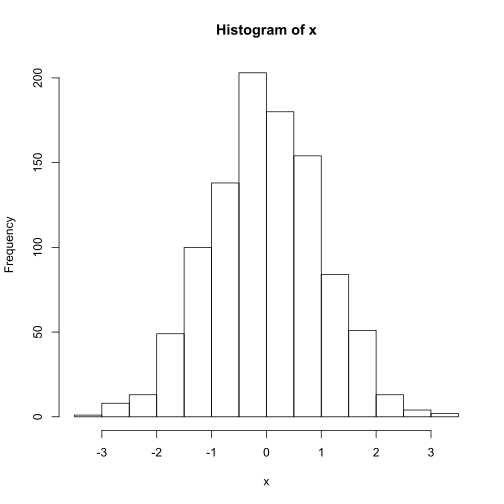
\includegraphics[width=0.7\textwidth]{figures/VIVIHist-1} \begin{Soutput}
This is a histogram, with the title: Histogram of x 
 "x" is marked on the x-axis.
Tick marks for the x-axis are at: -3, and 3 
There are a total of 1000 elements for this variable.
Tick marks for the y-axis are at: 0, 50, 100, 150, and 200 
It has 14 bins with equal widths, starting at -3.5 and ending at 3.5 .
The mids and counts for the bins are:
mid = -3.25  count = 1 
mid = -2.75  count = 8 
mid = -2.25  count = 13 
mid = -1.75  count = 49 
mid = -1.25  count = 100 
mid = -0.75  count = 138 
mid = -0.25  count = 203 
mid = 0.25  count = 180 
mid = 0.75  count = 154 
mid = 1.25  count = 84 
mid = 1.75  count = 51 
mid = 2.25  count = 13 
mid = 2.75  count = 4 
mid = 3.25  count = 2
\end{Soutput}
\end{Schunk}


Other functions exist for boxplots and dotplots. Try:
\begin{Schunk}
\begin{Sinput}
> VI(boxplot(x))
\end{Sinput}

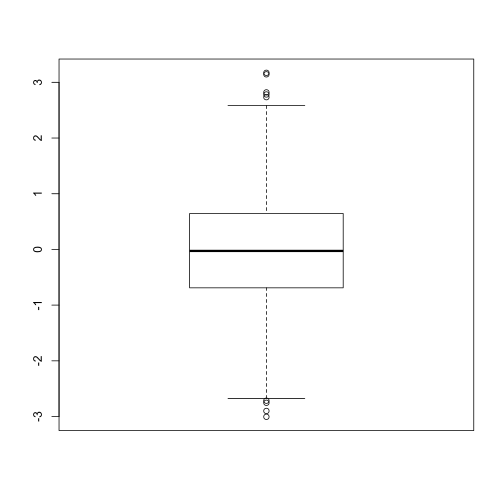
\includegraphics[width=0.7\textwidth]{figures/VIVIBoxplot-1} \begin{Soutput}
This graph has a boxplot printed vertically
but has no title
No label appears on the x-axis.
No label appears on the y-axis.
Tick marks for the y-axis are at: -3, and 3 
This variable has 1000 values.
An outlier is marked at: 3.171 2.782 2.819 3.144 -2.716 -2.753 2.733 -2.9 -3.005 
The whiskers extend to -2.676 and 2.583 from the ends of the box, 
which are at -0.6895 and 0.6447 
The median, -0.02724 is 50 % from the lower end of the box to the upper end.
The upper whisker is 0.98 times the length of the lower whisker.
\end{Soutput}
\end{Schunk}
 and
\begin{Schunk}
\begin{Sinput}
> VI(dotplot(x))
\end{Sinput}
\begin{Soutput}
Warning in dotplot.default(x): The dotplot command is a wrapper for stripchart, and is not a base R function.
\end{Soutput}

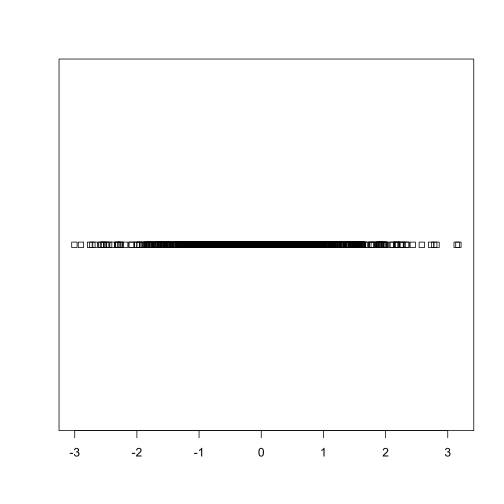
\includegraphics[width=0.7\textwidth]{figures/VIVIDotplot-1} \begin{Soutput}
This graph has a dotplot printed horizontally
but has no title
No label appears on the x-axis.
No label appears on the y-axis.
Tick marks for the x-axis are at: -3, and 3 
the data that range from -3.00520712717559 to 3.17125282201477 has been broken into 6 bins.
The counts are:
: 23 161 363 325 112 16 
\end{Soutput}
\end{Schunk}

The \Rcmd{dotplot} command is not part of base \R{} which uses the \Rcmd{stripchart} command instead. The \Rcmd{hist} and \Rcmd{boxplot} commands used here are actually commands from the \Rpkg{BrailleR} package that use the standard commands indirectly. At this point in time, I haven't worked out how to get the \Rcmd{stripchart} command to work as a \Rpkg{BrailleR} command so I needed to use a different name for my version. The \Rpkg{BrailleR} versions of these three commands store the additional information we need to get the text interpretation that is not possible from the standard version of the commands.


\section{Basic descriptions of variables}

The \Rcmd{UniDesc} function is designed to quickly generate a text summary of a single variable. It also saves several graphs. It can also save the text in a file and use the \Rcmd{VI} command from the \Rpackage{BrailleR} package to add text descriptions to the output file.

One obvious issue is that saving lots of files could become problematic. Default filenames are used and all files can be put into a folder of the user's choosing.

An example will help. Try
\begin{Schunk}
\begin{Sinput}
> data(airquality)
> Ozone=airquality$Ozone
> UniDesc(Ozone, Folder="AirQuality")
\end{Sinput}
\end{Schunk}
Take a look in the \file{AirQuality} folder that has been created in your working directory. It has a number of files that all start with ``Ozone" --- the name of the variable being analysed.  You will also have three files stored in the current working directory which have the filename \file{Ozone-UniDesc.*} where the star is for the extension which is one of \file{html}, \file{R}, and \file{Rmd}.

The most useful one at first is the \file{Ozone-UniDesc.html} file. Open this file in a browser to see what analyses have been included. This file is specifically formatted for use with screen readers. I hope you find it valuable. If you are reading this document on the web, then the link \url{Ozone-UniDesc.html} will open it in your browser. The link will not work if you are using the \file{pdf} version of LURN.

The commands used to generate parts of this HTML document are given in the \R{} script file; the third file is called an \R{} markdown document. This is the file that gets converted into the other two files. It might prove useful to learn how to write this kind of file for yourself one day.

In the \file{airquality} subfolder you will find that graphs have been saved in a variety of formats. They each have their uses and hopefully the filetype you need is there. Special attention is made for those users of \LaTeX{} who need specific formats for graphics. Some more advanced information is presented in \LaTeX{} formatted tables and put into files with the \file{tex} extension. For example, the content of Table~\ref{OzoneNormality} were presented in the \file{Ozone-UniDesc.html} document and included in this document using the \LaTeX{}version of that table.
\input{Ozone/Ozone-Normality}


Whenever the \Rcmd{VI} function is employed on an object that does not yet have an explicit function tied to it, then you will be told that this is the case. This package is a work in progress after all. Please feel free to send an email if you'd like any extra functionality.



\section{Altering \R{} output to make it easier to read}

Some \R{} output is arranged in nice tables that are easy for the sighted user to read, but are difficult to understand if using synthesised  speech to read the information back to you. The \Rcmd{VI} command is used again here but is now employed on a \Rclass{data.frame} object. We'll compare it with the \Rcmd{summary} command used frequently.
\begin{Schunk}
\begin{Sinput}
> summary(airquality)
\end{Sinput}
\begin{Soutput}
     Ozone          Solar.R         Wind      
 Min.   :  1.0   Min.   :  7   Min.   : 1.70  
 1st Qu.: 18.0   1st Qu.:116   1st Qu.: 7.40  
 Median : 31.5   Median :205   Median : 9.70  
 Mean   : 42.1   Mean   :186   Mean   : 9.96  
 3rd Qu.: 63.2   3rd Qu.:259   3rd Qu.:11.50  
 Max.   :168.0   Max.   :334   Max.   :20.70  
 NA's   :37      NA's   :7                    
      Temp          Month           Day      
 Min.   :56.0   Min.   :5.00   Min.   : 1.0  
 1st Qu.:72.0   1st Qu.:6.00   1st Qu.: 8.0  
 Median :79.0   Median :7.00   Median :16.0  
 Mean   :77.9   Mean   :6.99   Mean   :15.8  
 3rd Qu.:85.0   3rd Qu.:8.00   3rd Qu.:23.0  
 Max.   :97.0   Max.   :9.00   Max.   :31.0  
                                             
\end{Soutput}
\begin{Sinput}
> VI(airquality)
\end{Sinput}
\begin{Soutput}

The summary of each variable is
Ozone: Min. 1   1st Qu. 18   Median 31.5   Mean 42.1   3rd Qu. 63.2   Max. 168   NA's 37  
Solar.R: Min. 7   1st Qu. 116   Median 205   Mean 186   3rd Qu. 259   Max. 334   NA's 7  
Wind: Min. 1.7   1st Qu. 7.4   Median 9.7   Mean 9.96   3rd Qu. 11.5   Max. 20.7  
Temp: Min. 56   1st Qu. 72   Median 79   Mean 77.9   3rd Qu. 85   Max. 97  
Month: Min. 5   1st Qu. 6   Median 7   Mean 6.99   3rd Qu. 8   Max. 9  
Day: Min. 1   1st Qu. 8   Median 16   Mean 15.8   3rd Qu. 23   Max. 31  
\end{Soutput}
\end{Schunk}

The output generated by the \Rcmd{summary} command is difficult to follow as variables are represented in columns while rows that are read aloud by a screen reader are for the sample statistics.

The \Rcmd{VI} method has given us a summary of the variables one by one. This should prove easier to navigate and interpret as either a braille or screen reader user.

\section{Reading a scatter plot}


One challenge facing blind people is the inability to 
glance at a graph and understand what is intended just as sighted people can. The most difficult graphs to deal with are multidimensional representations of data. Two dimensional scatter plots are the first example of such graphs.

When a sighted person looks at a scatter plot, they are looking for a number of things. A relationship between the variables is the most common thing to look for, but there is also a need to identify points that are unusual in the context of the data presented.

One possible way to describe how the data points are summarised at a glance is that the graphing window is broken up into areas and a rough guess at the density of points within each region is evaluated. If this evaluation of density can be guessed, it can be counted more exactly by a purposely written function. The \Rcmd{WhereXY} function does this counting for us. It assumes equal-sized rectangular regions in the graph window. We can choose how many regions but the illustrations here all use a 5$\times$5 grid.

Let's work with a number of examples, all based on a set of predetermined $x$-values and various possible $y$-values.
\begin{Schunk}
\begin{Sinput}
> x=(0:100)/100
> y1=5*x+rnorm(101)
> y2=(2*x-1)^2+rnorm(101)/6
> y3=11*x+rnorm(101)
> y4=y3; y4[100]=0
\end{Sinput}
\end{Schunk}

What we might guess from the above is that a graph of $(x,y_1)$ pairs would show quite a lot of noise; $(x,y_2)$ pairs are a parabola with some noise; $(x,y_3)$ pairs are for a straight line with some noise; and, $(x,y_4)$ pairs are the same as the previous straight line, but one point is some distance from the line.

The \Rcmd{WhereXY} command for each plot is now given.
\begin{Schunk}
\begin{Sinput}
> WhereXY(x,y2, grid=c(5,5))
\end{Sinput}
\begin{Soutput}
     1  2  3  4  5 Sum
5    1  0  0  0  1   2
4    7  0  0  0  7  14
3   10  2  0  2 10  24
2    3 10  7 13  2  35
1    0  8 13  5  0  26
Sum 21 20 20 20 20 101
\end{Soutput}
\begin{Sinput}
> WhereXY(x,y2, grid=c(5,5))
\end{Sinput}
\begin{Soutput}
     1  2  3  4  5 Sum
5    1  0  0  0  1   2
4    7  0  0  0  7  14
3   10  2  0  2 10  24
2    3 10  7 13  2  35
1    0  8 13  5  0  26
Sum 21 20 20 20 20 101
\end{Soutput}
\begin{Sinput}
> WhereXY(x,y3, grid=c(5,5))
\end{Sinput}
\begin{Soutput}
     1  2  3  4  5 Sum
5    0  0  0  1 11  12
4    0  0  0 10  9  19
3    0  6 18  9  0  33
2   11 13  2  0  0  26
1   10  1  0  0  0  11
Sum 21 20 20 20 20 101
\end{Soutput}
\begin{Sinput}
> WhereXY(x,y4, grid=c(5,5))
\end{Sinput}
\begin{Soutput}
     1  2  3  4  5 Sum
5    0  0  0  1 10  11
4    0  0  0 10  9  19
3    0  6 18  9  0  33
2   11 13  2  0  0  26
1   10  1  0  0  1  12
Sum 21 20 20 20 20 101
\end{Soutput}
\end{Schunk}

We might also alter the number of cells in the grid to see how sensitive we want to make our investigation. Personal preferences will determine which combination of rows and columns works best.

\section{What else?}

Future developments in the BrailleR package will be made to meet demand. If you do want some additional functionality that you think is likely to be wanted by others then please do add to the wish list. Current ideas on the wish list include:
\begin{itemize}
\item Easier to interpret multiple regression output.
\item Easier to interpret principal component analysis output.
\item More graph types being described using the \Rcmd{VI} command.
\item Easier to interpret factor analysis output.
\end{itemize}




